\documentclass[a4paper, 12pt]{article}
\usepackage[utf8]{inputenc}
\usepackage[T2A]{fontenc}
\usepackage{amsmath,amssymb,amsthm}
\usepackage[a4paper,hmargin=2.5cm,vmargin=2.5cm]{geometry}
\usepackage[english]{babel}
% \usepackage{graphics}
\usepackage{float}
\usepackage{graphicx}


\DeclareMathOperator{\argmax}{argmax}
\DeclareMathOperator{\Image}{Im}


\graphicspath{{./images/}}

\theoremstyle{definition}
\newtheorem{definition}{Definition}[section]


\theoremstyle{definition}
\newtheorem{example}{Example}[section]

\newtheorem{theorem}{Theorem}

\theoremstyle{remark}
\newtheorem*{remark}{Remark}

\begin{document}

%%
%% Title page
%%
\begin{center}
{\scshape Federal State Autonomous Educational Institution\\
for the Higher Education\\
National Research University ``Higher School of Economics''\\[1ex]
Faculty of Mathematics\par}

\par\vfill

\textbf{\large Grachev Denis Vadimovich}

\vspace{1.5cm}

{\Large\bfseries
Clustering of Multidimensional Random Variables \\ to Improve HMM Sequence Alignment Accuracy
\par}

\vspace{1.5cm}

\textbf{\large Project proposal}

\vspace{1cm}

% Field of study: 01.03.01 "--- Mathematics,\\[1ex]
% Degree programme: bachelor's educational programme ``Mathematics''
\par\vfill
\noindent\parbox[t]{0.48\textwidth}{%
Scientific supervisor:\\[3pt]
Prodanov Timofey Petrovich
}
% \hspace{0.04\textwidth}\parbox[t]{0.48\textwidth}{%
% Scientific supervisor:\\[3pt]
% Doctor of Sciences, professor\\
% Sergey Sergeevich Semyonov\\[2ex]
% }
\par\vfill\vfill
Moscow 2022
\end{center}
\thispagestyle{empty}
\pagebreak
%%
%% ===========================================================================
%%

\tableofcontents
\newpage

\section{Introduction}
Bioinformatics is an interdisciplinary science that aims 
to develops methods and software tools 
for understanding biological data. 
One of the ways to model haploid genome is to present it as 
pair of sequences or strings over the alphabet $\{ A, C, G, T \}$. 
Modern technologies of reading genome do not sequence it as one 
continious string, but a number of random overlaping substrings 
that are called reads. 
As within one biological species genomes coincide almost completely, 
it is convenient to determine one reference genome for one species 
and identify for every individual deviations from reference.
These single nucleotide variants are called SNVs.  

Taking into cosideration these facts and the fact that various 
errors happen during all stages of the process, a number of 
problems appears for example:
\begin{itemize}
    \item \textbf{Genome assembly} is process of  
    deciphering genome using reads obtained from it.
    
    \item \textbf{Sequence alignment} is process of 
    arranging sequences to spot similarities between them. 
    
    \item \textbf{Variant calling} is process of identifying 
    SNVs of an individual based on reads aligned on reference genome.
\end{itemize}

The most commonly used technologies nowadays, 
such as illumina, allow to sequence reads of length 200-500 bp.
Sequencing human genome using such short length reads 
has many limitations. 
First, due to diploidy of humans, it is important to obtain
long-range haplotype information. This might be difficult 
with short-reads provided by illumina. Secondly $~3.6\%$ of 
human genome consists of long highly repetative 
duplicated regeions that can not be uniquely aligned, 
which lowers accuracy of SNVs. 
Third-generation single-molecule sequencing techologies 
genereate longer reads of length 10-30 kb. 
This techology might help overcome limitations that 
short-reads have. Tools that use 

\newpage
\section{Methods}
\subsection{Clustering}

Given $X = \{x_i | x_i \in \mathbb{R}^d, i \in \left( 1 \ldots n \right) \}$ and $m \in \mathbb{N}$,
where $n$ is the number of points, $m$ - number of clusters. \\
Clustering algorithm takes $X$ and $m$ and outputs $C = \{ c_i | c_i \in \left( 1 \ldots m \right), i \in \left( 1 \ldots n \right)\}$.

\begin{figure}[H]
    
\includegraphics{example_clustering}
    \centering
    \caption{Example of clustering for $d=2$, $m=2$, color represents class.}
\end{figure}

\subsection{Strings}

\begin{definition}
    String of length $l$ over alphabet $A = \{ 1 \ldots m \}$ is a map $s: \{ 1 \ldots l\} \rightarrow A$.
    Usually elements of $A$ are denoted as characters for convenience.
\end{definition}

\begin{definition}
    Alignment of strings $s_1$ and $s_2$ of lengths $l_1$ and $l_2$ respectively, 
    over alphabet $A$ is a pair of strings $\hat{s}_1$ and $\hat{s}_2$ 
    of length $l$ over alphabet $A \sqcup \{ - \}$, 
    such that there exists increasing functions $f_i: \{1 \ldots l_i \} \rightarrow \{ 1 \ldots l\}$ 
    such that $\hat{s}_i|_{\hat{s}_i^{-1} (A)} \circ f_i = s_i$.
\end{definition}

\begin{remark}
    $\Image (f_i) = \hat{s}_i^{-1}(A)$
\end{remark}

\begin{example}
    Alignment of strings $s_1 = CABCAABA$ and $s_2 = ABADBBAD$ 
    over alphabet $\{ A, B, C, D\}$.

    \begin{center}
        \begin{tabular}{|| c | c c c c c c c c c ||}
         $s_1$ & C & A & B & C & A & A & B & A & \\ 
         $s_2$ & A & B & A & D & B & B & A &   & \\  
         $\hat{s}_1$ & C & A & B & C & - & A & A & B & A \\ 
         $\hat{s}_2$ & - & A & B & - & A & D & B & B & A   
        \end{tabular}
    \end{center}
\end{example}

\begin{definition}
    For given matrix $G \in \mathbb{R}^{|A| \times |A|}$ and $p \in \mathbb{R}$ 
    score of alignment $\hat{s}_1, \hat{s}_2$ is 
    $$ S(\hat{s}_1, \hat{s}_2) = \sum_{i = 1}^l \delta_i, 
        \text{ where } 
        \delta_{i}=
            \left\{\begin{array}{cc}
            g_{\hat{s}_1(i) \hat{s}_2(i)},& \hat{s}_1(i) \neq - \text{ and } \hat{s}_2(i) \neq -\\
            p, & 
            \end{array}\right. 
    $$
\end{definition}


\begin{theorem}
    If $G$ is symmetric and 
    $
    g_{ij} =
        \left\{\begin{array}{cc}
        0, & i = j\\
        >0, & 
        \end{array}\right.
    $ and $p > 0$, then we can define metric for strings over alphabet $A$ as 
    $$ d(s_1, s_2) = \min \{S(\hat{s}_1, \hat{s}_2)\}$$ 
\end{theorem}

\begin{proof}
    
\end{proof}

\begin{definition}
    For a string $s$ of length $l$, sub-string $s_s$ 
    is a string of length $l_s$, such that there exists an function
    $$f: \{ 1 \ldots l_s \} \rightarrow \{ 1 \ldots l\}$$
    $$f(i) = i + d $$
    $$s \circ f = s_s $$
\end{definition}

\begin{definition}
    For a string $s_1$ and $s_2$ of lengths $l_1, l_2$ correspondingly, define string-sub-string score as 
    $$ S_s (s_1, s_2) = \min \{ S(s_s, s_2) | s_s \text{ is a sub-string of } s \}$$

    and corresponding alignment $\hat{s}_1, \hat{s}_2$ 
    are pair of strings of lengths $l$ over alphabet $A \sqcup \{ - \}$
    such that there exists increasing functions 
    $f_1: \{1 \ldots l_1 \} \rightarrow \{ 1 \ldots l\}$
\end{definition}

\begin{definition}
    For a string $s$ of length $l$ and set of strings $R = \{ s_1 \ldots s_n \}$ 
    of lengths $\{ l_1 \ldots l_n \}$ correspondingly, 
    multiple alignment is tuple $\hat{s}, \hat{s}_1 \ldots \hat{s}_n$, 
    of strings of length $l$ over alphabet $A \sqcup \{ - \}$, such that $\sum_{i = 1}^n S(\hat{s}, \hat{s}_i)$ is minimal.
\end{definition}

\begin{definition}
    Set of reads $R$ for string $s$ of length $l$ and rate $r$ is 
    $$ R = \{ s_s | \text{length of } s_s > l, S_s(s, s_s) < r \}$$
\end{definition}

\section{Task}
Given reference string $s_r$ and reads $R$ for an unknown target string $s_t$, 
we know that $S(s_r, s_t) < D$ and whant to find $s_t$. \\

Plan:
\begin{enumerate}
    \item Make multiple alignment of $R$ over $s_r$.
    \item Estimate most likely difference between $s_r$ and $s_t$.
\end{enumerate}

\begin{figure}[H]
    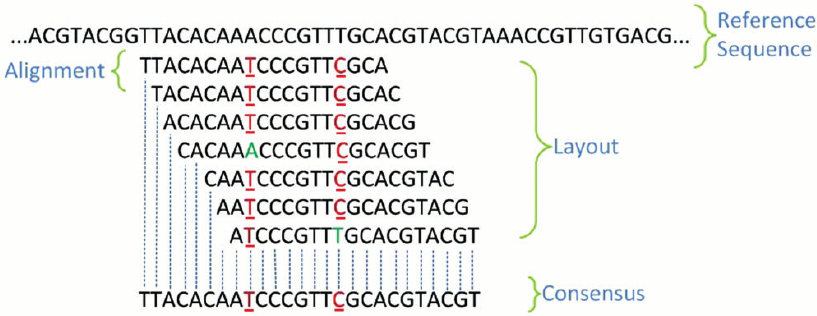
\includegraphics[scale=0.5]{aligned_reads.png}
    \centering
    \caption{Example of reference string, target string and reads.}
\end{figure}



\end{document}

